\documentclass[10pt,twocolumn,letterpaper]{article}
\usepackage[margin=1in,columnsep=0.25in]{geometry}
\usepackage[T1]{fontenc}
\usepackage{mathptmx,microtype}
\usepackage{amsmath,amssymb,booktabs,array,graphicx,xcolor}
\usepackage{listings,tikz}
\usepackage[hidelinks]{hyperref}
\usepackage[font=small,labelfont=bf]{caption}
\definecolor{accent}{RGB}{34,65,92}
\definecolor{codebg}{RGB}{247,248,250}
\lstset{basicstyle=\ttfamily\scriptsize,keywordstyle=\color{accent}\bfseries,
 commentstyle=\color{gray},stringstyle=\color{accent},backgroundcolor=\color{codebg},
 breaklines=true,columns=fullflexible,keepspaces=true,showstringspaces=false,
 numbers=left,numberstyle=\tiny\color{gray},numbersep=7pt,frame=single,
 rulecolor=\color{black!15},xleftmargin=12pt,aboveskip=9pt,belowskip=9pt,
 captionpos=b}
\raggedbottom
\urlstyle{same}
\setlength{\parindent}{0pt}
\setlength{\parskip}{4pt}
\setlength{\emergencystretch}{1.5em}
\newcommand{\pending}[2]{\begin{center}\fbox{\parbox{0.90\linewidth}{\centering
\vspace{5pt}\textbf{#1}\\[4pt]\small #2\vspace{5pt}}}\end{center}}
\newcommand{\code}[1]{\texttt{\detokenize{#1}}}
\makeatletter
\renewcommand{\maketitle}{\begin{center}
\hrule height 3pt\vspace{9pt}
{\Large\bfseries\@title\par}\vspace{8pt}\hrule height 0.5pt\vspace{10pt}
\@author\par\vspace{8pt}
{\small EE224 Digital Systems $\cdot$ Course Project $\cdot$ Semester 1, 2026--2027}
\end{center}\vspace{6pt}}
\makeatother
\title{Implementing Convolutional Neural Network Inference\\Through a $4\times4$ Systolic Array}
\author{\begin{tabular}{ccc}
\textbf{Ayush Agrawal} & \textbf{Rajveer Singh Choudhary} & \textbf{Atharva Airen}\\[5pt]
25B1304 & 25B1313 & 25B1207\\[6pt]
{\small Python; PE RTL} & {\small Python; array RTL} & {\small Testbenches; report}
\end{tabular}}
\begin{document}
\twocolumn[\maketitle
\begin{center}\begin{minipage}{0.92\textwidth}
\begin{center}\textbf{Abstract}\end{center}
We implement a signed multiply--accumulate processing element and connect sixteen
instances into a structural $4\times4$ systolic array. Input skew aligns the
operands of each dot product while each processing element retains its own
partial sum. We derive full-array latencies of 10 and 14 active clock edges for
$4\times4$ by $4\times4$ and $4\times8$ by $8\times4$ multiplication,
respectively. A two-convolution MNIST classifier is converted to signed integer
matrix operations and mapped to the same array using output tiling. Saved
notebook evaluation reports 98.52\% training and 98.33\% test accuracy.
Self-checking testbenches cover the processing element, matrix operations, and
100 balanced CNN inputs. Local behavioural simulation verifies the PE and both matrix cases, including
all output entries and the derived latencies. Recorded waveforms accompany
archived Python evidence and a teammate-provided ModelSim CNN waveform.
The supplied ModelSim summary reports 99 correct predictions out of 100,
zero matrix-product mismatches, and complete agreement with its NumPy
integer reference.
\end{minipage}\end{center}\vspace{10pt}]

\section{Scope and evidence}
The report follows Parts A, B(i), B(ii), C(i), and C(ii) of the EE224 question
paper~\cite{question}. The implementation is based on the local working copy
of the course repository~\cite{repo}, whose Git base is commit \code{70a34f2},
with local RTL fixes, testbenches, and additional notebook exports.

The two synthesizable modules are \code{processing_element.v} and
\code{systolic_array.v}. Stimulus generation, matrix tiling, activation,
pooling, and classification are testbench operations. The three testbench tops
have compiled successfully with Icarus Verilog 12.0. The PE and array benches
were also executed locally: every assertion passed, including the additional
partial-tile and long-dot-product cases. The recorded VCD traces independently
confirm all sixteen entries of both required products and the completion
edges. Figures are rendered from those VCD events, rather than recreated
from theoretical timing. Separate teammate-provided ModelSim waveform and transcript screenshots
are included as Part C evidence. It is not a run of the local CNN bench.
No new training run or local CNN simulation is claimed.

\subsection*{Contributions}
Ayush Agrawal and Rajveer Singh Choudhary developed the Python code.
All three members contributed to Verilog: Ayush implemented the processing
element, Rajveer implemented the systolic array, and Atharva Airen worked on
the testbenches. Atharva prepared the report.

\section{Part A: Processing element}
\subsection{Operation and implementation}
The processing element (PE) has two $W$-bit inputs, two registered forwarding
outputs, and one accumulator. In the question paper's interval notation,
\begin{align}
a_{\mathrm{out}}(t)&=a_{\mathrm{in}}(t-1),\\
b_{\mathrm{out}}(t)&=b_{\mathrm{in}}(t-1),\\
c_{\mathrm{out}}(t)&=c_{\mathrm{out}}(t-1)
 +a_{\mathrm{in}}(t-1)b_{\mathrm{in}}(t-1).
\end{align}
Here the inputs on the right are stable just before the rising edge, and the
outputs on the left are sampled after the register updates settle. On an
active-high reset, all three registers clear asynchronously.

Appendix~\ref{app:rtl} contains the complete RTL. Nonblocking
assignments ensure that neighboring PEs consume the previous registered
forwarding values at an edge. The input product uses the current external
inputs, rather than the already delayed forwarding outputs. There is no
clock enable: a zero product holds the sum; reset begins a new dot product.

\subsection{Signed representation and width}
The design uses $W=8$ signed two's-complement operands, supporting integers
in $[-128,127]$, because trained weights may be negative. A separate signed
$2W$-bit wire represents the full product. The accumulator width is 24 bits.
The longest CNN dot product has 250 terms, with the conservative bound
\begin{equation}
|s|\leq250\,(128)^2=4{,}096{,}000.
\end{equation}
This bound fits in 23 signed bits; choosing 24 provides additional headroom.
A signed 16-bit sum, limited to $[-32{,}768,32{,}767]$, is insufficient.
Bias addition takes place separately in 32-bit testbench arithmetic.

\subsection{Testbench and expected behaviour}
\code{tb_processing_element.sv} applies operands at falling edges, samples
outputs 1\,ns after rising edges, and checks forwarding and the accumulated
sum. Table~\ref{tab:pe} gives the initial expected sequence. Reset is also
asserted after a nonzero sum, verifying that it clears accumulated state.
Two additional sequences accumulate 250 copies of $(-128)(-128)$ and
$(-128)(127)$, giving $4{,}096{,}000$ and $-4{,}064{,}000$ respectively.

\begin{table}[t]\centering\small
\caption{PE reference values after successive active edges. Expected values, also verified against the recorded PE waveform.}\label{tab:pe}
\begin{tabular}{rrrr}\toprule
Step & $a_{\rm in}$ & $b_{\rm in}$ & $c_{\rm out}$\\\midrule
Reset & 0 & 0 & 0\\
1 & 3 & 4 & 12\\
2 & $-5$ & 7 & $-23$\\
3 & $-128$ & $-128$ & 16,361\\
4 & 127 & $-128$ & 105\\
5 & 0 & 127 & 105\\\bottomrule
\end{tabular}
\end{table}
\begin{figure*}[t]\centering
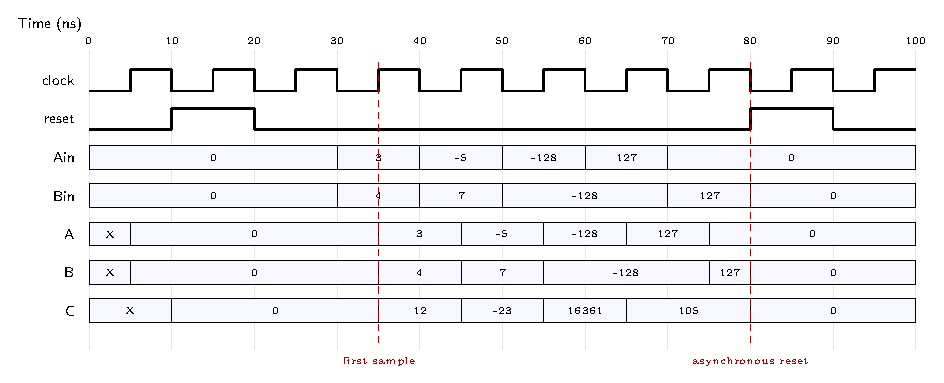
\includegraphics[width=\textwidth]{figures/pe_waveform.pdf}
\caption{Part A: recorded PE waveform. Signed decimal buses show forwarding, negative products, accumulation, and asynchronous reset at 80 ns. The 250-term checks also pass in the full simulation log.}\label{fig:pe_waveform}
\end{figure*}

\section{Part B: Structural systolic array}
\subsection{Connections and dataflow}
Sixteen instances form a $4\times4$ grid (Figure~\ref{fig:array}). The $A$
operand moves right by one PE per edge; the $B$ operand moves down by one PE
per edge. Each PE retains the sum for one output matrix entry. This is an
output-stationary organization. For output row $i$ and column $j$,
\begin{equation}
C_{ij}=\sum_{q=0}^{K-1}A_{iq}B_{qj},\quad 0\leq i,j<4.
\end{equation}
The HDL uses nested generate loops. Packed input lane $i$ occupies bits
$[8i+7:8i]$; output $C_{ij}$ occupies the 24-bit field starting at
$24(4i+j)$. Top-level forwarding outputs connect to the right and bottom
boundaries. Only one definition of the PE is compiled.

\begin{figure}[t]\centering
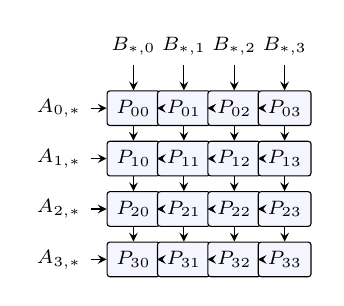
\begin{tikzpicture}[x=0.64cm,y=0.64cm,>=stealth,
 every node/.style={font=\scriptsize}]
\foreach \i in {0,...,3}{\foreach \j in {0,...,3}{
\node[draw,rounded corners=1pt,fill=blue!4,minimum width=.53cm,minimum height=.44cm] (p\i\j) at (\j,-\i) {$P_{\i\j}$};}}
\foreach \i in {0,...,3}{\foreach \j [evaluate=\j as \k using int(\j+1)] in {0,...,2}{
\draw[->] (p\i\j)--(p\i\k);}}
\foreach \i [evaluate=\i as \k using int(\i+1)] in {0,...,2}{\foreach \j in {0,...,3}{
\draw[->] (p\i\j)--(p\k\j);}}
\foreach \i in {0,...,3}{\draw[->] (-.85,-\i) node[left] {$A_{\i,*}$} -- (p\i0);}
\foreach \j in {0,...,3}{\draw[->] (\j,.85) node[above] {$B_{*,\j}$} -- (p0\j);}
\end{tikzpicture}
\caption{Structural $4\times4$ array. Each node stores one partial output sum. Input streams are skewed before entering the grid.}\label{fig:array}
\end{figure}

\subsection{Input schedule and latency derivation}
Let $t=0$ denote the first active sampling edge. The driver supplies
\begin{align}
a_i[t]&=\begin{cases}A_{i,t-i},&0\leq t-i<K,\\0,&\text{otherwise},\end{cases}\\
b_j[t]&=\begin{cases}B_{t-j,j},&0\leq t-j<K,\\0,&\text{otherwise}.\end{cases}
\end{align}
Row $i$ and column $j$ are delayed by $i$ and $j$ edges. Hence operands with
inner index $q$ meet at PE $(i,j)$ on zero-based edge $t=q+i+j$.
Counting the first sampling edge as edge 1, the last term at that PE is
accumulated on edge $K+i+j$. PE $(3,3)$ finishes last, so
\begin{equation}\boxed{L=K+6\text{ active clock edges}.}\label{eq:latency}\end{equation}
This is the generic latency of this architecture and specified streaming
schedule, excluding reset/setup and subsequent reading of registers.
It assumes the full product is required and does not exploit known zeros.
It is not a measured wall-clock runtime.

\subsection{\texorpdfstring{Part B(i): $4\times4$ by $4\times4$}{Part B(i): 4x4 by 4x4}}
For $K=4$, Equation~\ref{eq:latency} gives \textbf{10 active edges}.
PE $(0,0)$ receives its last term on edge 4, whereas PE $(3,3)$ starts on
edge 7 and finishes on edge 10. Sampling the full matrix at edge 4 would
therefore be premature.

The first case in \code{tb_systolic_array.sv} uses $M=N=K=4$ and seed
$s=1$. Its operands are defined reproducibly by
\begin{align}
A_{rq}&=((29r+7q+s)\bmod256)-128,\\
B_{qc}&=((11q+31c+3s)\bmod256)-128.
\end{align}
The independently computed reference output is
{\scriptsize\begin{equation*}
C_4=\begin{bmatrix}
50946&36500&22054&7608\\38360&27510&16660&5810\\
25774&18520&11266&4012\\13188&9530&5872&2214
\end{bmatrix}.
\end{equation*}}
All sixteen recorded entries match this reference. The first sampling edge
is at 35\,ns and the complete matrix appears at 125\,ns: ten rising edges
counted inclusively. The bottom-right entry is still incomplete one edge
earlier. The complete operands are in Appendix~\ref{app:matrices}.
The shared driver checks every PE's partial sum on every active edge and
compares all final entries against scalar multiplication.
\begin{figure*}[t]\centering
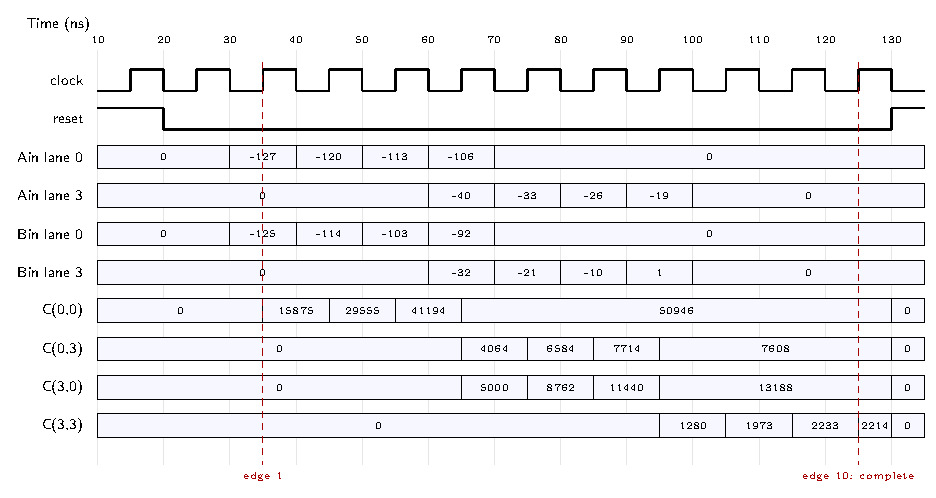
\includegraphics[width=\textwidth]{figures/array_k4_waveform.pdf}
\caption{Part B(i): recorded input lanes and representative accumulators. The first input is sampled at 35 ns (edge 1), and all sixteen outputs match the reference at 125 ns (edge 10). Lane 3 illustrates the input skew.}\label{fig:array_k4_waveform}
\end{figure*}

\subsection{\texorpdfstring{Part B(ii): $4\times8$ by $8\times4$}{Part B(ii): 4x8 by 8x4}}
The same hardware accepts eight terms in each dot product. Only the stream
length changes: there are still sixteen PEs, and each accumulates eight
products. For $K=8$, the full matrix requires \textbf{14 active edges}.
The testbench's second case uses $s=9$, producing the reference
{\scriptsize\begin{equation*}
C_8=\begin{bmatrix}
50484&27048&3612&-19824\\35984&19740&3496&-12748\\
21484&12432&3380&-5672\\6984&5124&3264&1404
\end{bmatrix}.
\end{equation*}}
All sixteen recorded entries match this reference. Sampling begins at
155\,ns and completes at 285\,ns, giving fourteen active rising edges
counted inclusively. The bottom-right entry is incomplete on the preceding
edge. The driver resets all accumulators between products. Further cases exercise
zero operands after a nonzero product, signed values, partial output tiles,
and $K=9,45,250,128$. Appendix~\ref{app:tests} contains the testbenches.
\begin{figure*}[t]\centering
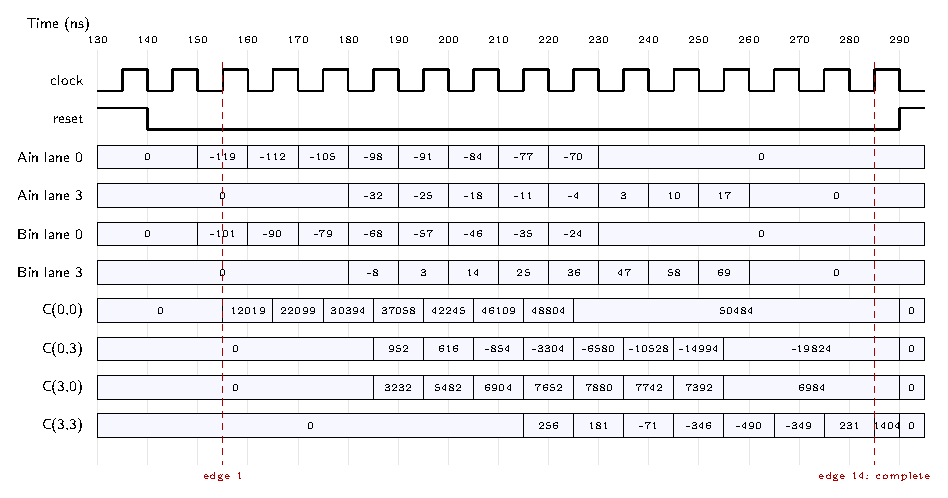
\includegraphics[width=\textwidth]{figures/array_k8_waveform.pdf}
\caption{Part B(ii): recorded input lanes and representative accumulators. Sampling starts at 155 ns (edge 1), and all sixteen outputs match the reference at 285 ns (edge 14).}\label{fig:array_k8_waveform}
\end{figure*}

\section{Part C(i): CNN training on MNIST}
\subsection{Architecture and training procedure}
The Keras notebook implements the question paper's architecture
(Table~\ref{tab:cnn}). MNIST has 60,000 training and 10,000 test images,
each $28\times28$ and grayscale. Pixel values are normalized by 255;
labels are one-hot encoded into ten classes. Both convolutions use $3\times3$
kernels, stride 1 and valid padding. Both pooling layers use valid $2\times2$
windows and stride 2.

The saved notebook trains for five epochs using Adam with learning rate
$10^{-3}$, categorical cross-entropy, and the Keras default batch size of
32. The test split is supplied for validation during fitting and then
explicitly evaluated. Dropout is 0.45 during training and inactive during
inference. The PyTorch script is an alternate training implementation;
the reported numbers and integer exports here refer to the Keras notebook.

\begin{table}[t]\centering\small
\caption{CNN architecture. Shapes exclude the batch dimension.}\label{tab:cnn}
\begin{tabular}{lrr}\toprule
Layer & Output shape & Parameters\\\midrule
Input & $28\times28\times1$ & 0\\
Conv1 + ReLU & $26\times26\times5$ & 50\\
Max pool 1 & $13\times13\times5$ & 0\\
Conv2 + ReLU & $11\times11\times10$ & 460\\
Max pool 2 & $5\times5\times10$ & 0\\
Flatten; dropout & 250 & 0\\
Dense1 + ReLU & 128 & 32,128\\
Dense2 + softmax & 10 & 1,290\\\midrule
Total & & 33,928\\\bottomrule
\end{tabular}
\end{table}

\subsection{Training and test accuracy}
Figures~\ref{fig:train} and \ref{fig:test} reproduce the plots embedded in the
saved notebook; they were not generated by a new run for this report.
Final explicit evaluation records
\begin{align*}
\text{training accuracy}&=98.5217\%,\\
\text{test accuracy}&=98.3300\%.
\end{align*}
Both exceed the required 80\% threshold. The final epoch's plotted training
accuracy is approximately 96.27\%, measured while training with dropout and
changing weights. The final training-set evaluation is higher because it
uses fixed final weights and inference mode. These are different metrics,
so the plot endpoint should not be relabeled as 98.52\%.

The test set is reused as validation data in the supplied notebook. Its
reported accuracy is the course-required train/test result; this setup does
not provide a separate validation split for independent model selection.

\begin{figure}[t]\centering
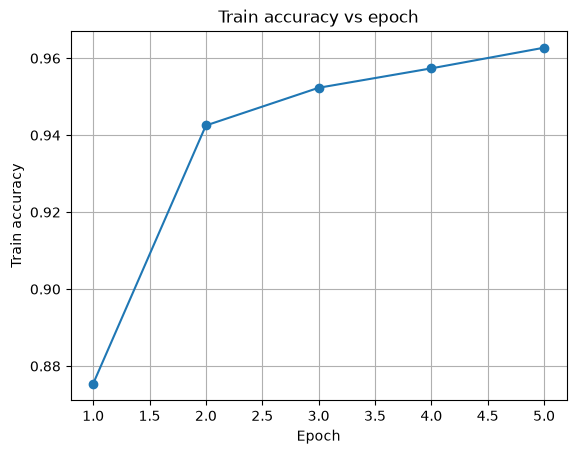
\includegraphics[width=\linewidth]{figures/train_accuracy.png}
\caption{Saved training accuracy versus epoch, recorded during fitting with dropout active.}\label{fig:train}
\end{figure}
\begin{figure}[t]\centering
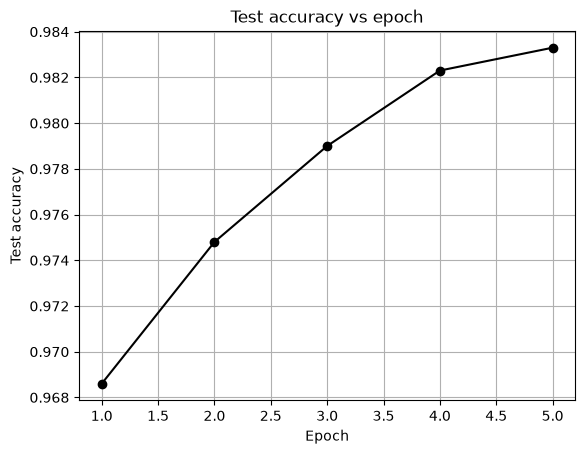
\includegraphics[width=\linewidth]{figures/test_accuracy.png}
\caption{Saved test/validation accuracy versus epoch. The final value is 98.33\%.}\label{fig:test}
\end{figure}

\section{Part C(ii): Integer CNN inference}
\subsection{Weight extraction and fixed-point format}
The notebook extracts kernels and biases using each Keras layer's
\code{get_weights()} method. Convolution kernels are reshaped from
$(3,3,C_{\rm in},C_{\rm out})$ into matrices
$(9C_{\rm in},C_{\rm out})$, preserving NHWC patch order. Dense kernels
already have the required input-feature by output-feature layout.

Define $\operatorname{sat}_{l,u}(z)=\min(u,\max(l,z))$. The integer encoding is
\begin{align}
x_q&=\operatorname{sat}_{-128,127}(\operatorname{round}(2^6x)),\\
w_q&=\operatorname{sat}_{-128,127}(\operatorname{round}(2^7w)),\\
b_q&=\operatorname{round}(2^{13}b).
\end{align}
Input images lie in $[0,1]$, so their encoded pixels lie in $[0,64]$.
Weights use signed 8-bit storage, biases use 32-bit integers, and raw matrix
products use 24-bit DUT accumulators. A bias has the same scale as the
product of a Q6 activation and a Q7 weight.

For convolution and Dense1, the next activation is
\begin{equation}
y_q=\operatorname{sat}_{0,127}\big((\sum x_qw_q+b_q)\mathbin{\ggg}7\big).
\end{equation}
The signed arithmetic shift returns the result to scale $2^6$; clipping
implements ReLU and saturation. This matches the notebook's integer right
shift rather than introducing an additional rounding operation. Quantization
can clip weights and activations, so a separate integer evaluation is
necessary. Dense2 produces logits; their argmax gives the class without
computing softmax, which preserves the ordering of logits.

\subsection{Grayscale convolution as multiplication}
For an $H\times W\times C_{\rm in}$ activation tensor, unfold every valid
$3\times3$ patch into a row of length $9C_{\rm in}$. Patches are ordered by
output row, output column, kernel row, kernel column, and channel. If
$P=(H-2)(W-2)$, the convolution becomes
\begin{equation}
\underbrace{X_{\rm col}}_{P\times9C_{\rm in}}
\underbrace{W_{\rm col}}_{9C_{\rm in}\times C_{\rm out}}
=\underbrace{G}_{P\times C_{\rm out}}.
\end{equation}
Bias is added by output channel after the multiplication. For the grayscale
first layer, $C_{\rm in}=1$ and each patch has nine entries, rather than the
27 entries of a $3\times3\times3$ RGB patch. Conv2 acts on five feature
channels, so its patch length is 45, despite the original image being
grayscale.

\begin{table*}[t]\centering\small
\caption{Per-image matrix mapping and derived active-edge budget for the current driver. Each output tile receives a fresh reset. Setup/reset edges are excluded; these values are not simulator measurements.}\label{tab:mapping}
\begin{tabular}{lrrrrr}\toprule
Layer & $X$ shape & $W$ shape & Output tiles & Edges/tile & Active edges\\\midrule
Conv1 & $676\times9$ & $9\times5$ & $169\cdot2=338$ & 15 & 5,070\\
Conv2 & $121\times45$ & $45\times10$ & $31\cdot3=93$ & 51 & 4,743\\
Dense1 & $1\times250$ & $250\times128$ & $1\cdot32=32$ & 256 & 8,192\\
Dense2 & $1\times128$ & $128\times10$ & $1\cdot3=3$ & 134 & 402\\\midrule
Total per image & & & 466 & & 18,407\\\bottomrule
\end{tabular}
\end{table*}

\subsection{Tiling and layer-to-layer execution}
Table~\ref{tab:mapping} shows the four matrix products for one image. A
matrix product $M\times K$ by $K\times N$ is partitioned into
$\lceil M/4\rceil\lceil N/4\rceil$ output tiles. Each tile streams all $K$
terms through the array; the inner dimension is not restricted to four.
Unused rows and columns in a boundary tile receive zeros, and only valid
entries are retained. Reset prevents sums from leaking between tiles.
The driver deliberately uses the full $K+6$ schedule even for partial tiles.

The CNN bench processes each image through Conv1, requantization/ReLU,
$2\times2$ max pooling, Conv2, requantization/ReLU, another max pool,
flattening, Dense1, and Dense2. Pooling reduces the second convolution's
$11\times11$ spatial output to $5\times5$, dropping the final unmatched row
and column. Flattening follows Keras NHWC order. Every convolution and dense
matrix product uses actual DUT outputs. The surrounding operations execute
in the testbench, with each subsequent layer constructed from the previous
DUT results. Golden matrices are used only for comparison.

The notebook also exports goldens using batch-stacked rows. Those batch
matrices have shapes $67600\times9$, $12100\times45$, $100\times250$, and
$100\times128$ on the left. Their padded row grouping is distinct from the
per-image hardware schedule, but the bench reads each image's golden rows
in order. Batch export tile counts must not be substituted for the
per-image counts in Table~\ref{tab:mapping}.

\subsection{Balanced evaluation and correctness checks}
The notebook chooses the first ten test examples for each label 0--9,
yielding 100 balanced samples. Images, all weights and biases, labels,
expected predictions, and four golden matrix products are exported together
into \code{modelsim_data}. The bench rejects missing or malformed values,
values outside their supported ranges, trailing data, and an unbalanced
label distribution.

For each tile, an independent scalar scoreboard checks every partial MAC
sum on every edge. The CNN bench also compares all final matrix entries
against exported NumPy goldens and verifies predictions against the integer
reference. Accuracy is calculated from the true labels:
\begin{equation}
\operatorname{Accuracy}=\frac{1}{100}\sum_{n=1}^{100}
\mathbf{1}\{\widehat y_n=y_n\}\times100\%.
\end{equation}
Accuracy is reported even if it is below the floating-point result; it is
not replaced by agreement with the golden predictions. Incorrect reference
predictions still count as classification errors.

\begin{table}[t]\centering\small
\caption{Recorded results and their evidence sources.}\label{tab:status}
\begin{tabular}{@{}p{0.61\linewidth}p{0.29\linewidth}@{}}\toprule
Quantity & Result / status\\\midrule
Floating-point training, 60,000 & 98.52\% (saved)\\
Floating-point test, 10,000 & 98.33\% (saved)\\
Integer Python test, balanced 100 & 98/100 (saved)\\
DUT-based test, balanced 100 & \textbf{99/100 (99\%)}\\
Behavioural PE/matrix evidence & \textbf{Passed locally}\\\bottomrule
\end{tabular}
\end{table}
The saved second notebook cell reports 98/100 for Python integer inference.
That cell has no execution count, so this is an archived output rather than
a newly reproduced measurement. It is not a Verilog simulation result.
The teammate's ModelSim run instead reports 99/100 classification accuracy
and 100/100 agreement with its NumPy integer model. Its corresponding
NumPy predictions therefore also achieve 99/100 in that run. The older
98/100 notebook output and the supplied simulator result document separate
run artifacts; their difference is not a hardware mismatch. The model
weights and exported inputs of the teammate's run have not been reconciled
with the archived notebook. The report retains their separate provenance
rather than attributing both scores to one identical experiment.

\subsection{Teammate-provided CNN simulation evidence}
Figure~\ref{fig:cnn_modelsim} reproduces the supplied ModelSim waveform
from a separate testbench named \code{tb_cnn}. It shows clock, reset,
packed operands, accumulated results, matrix dimensions, and error/cycle
counters. In the visible early waveform interval the dimensions are
$M=67{,}600$, $K=9$, $N=8$, consistent with the batch-stacked, column-padded
Conv1 export. The value column shows $M=12{,}100$, $K=45$, $N=12$,
consistent with the corresponding Conv2 export at the selected state.
Both \code{errors} and \code{total_errors} are displayed as zero.

The final simulator transcript in Figure~\ref{fig:cnn_summary} supplies the
completed-run evidence. Its reported results are:
\begin{itemize}
\item Total matrix-product mismatches against NumPy golden: \textbf{0}.
\item Total clock cycles, all layers: \textbf{1,228,425}.
\item Systolic-array test accuracy: \textbf{99/100 (99\%)}.
\item Agreement with the NumPy integer model: \textbf{100/100}.
\end{itemize}
The visible transcript lists labels and predictions through image 99 and
then terminates with \code{$finish} in \code{Testbench2.v}. The final
matrix dimensions shown are $M=100$, $K=128$, $N=12$, consistent with the
batch-stacked Dense2 operation with output columns padded from ten to twelve.
The complete agreement and zero matrix mismatches show that the simulated
matrix operations match the supplied reference for this run. The one
classification error is also made by that reference model.

The reported aggregate cycle count belongs to the teammate's batched
\code{tb_cnn} implementation. It is not substituted for the per-image
schedule of the local driver in Table~\ref{tab:mapping}; the schedules
use different tile groupings and counter conventions. The screenshot is
provided evidence of the teammate's run, not a newly executed local CNN run.

\begin{figure*}[p]\centering
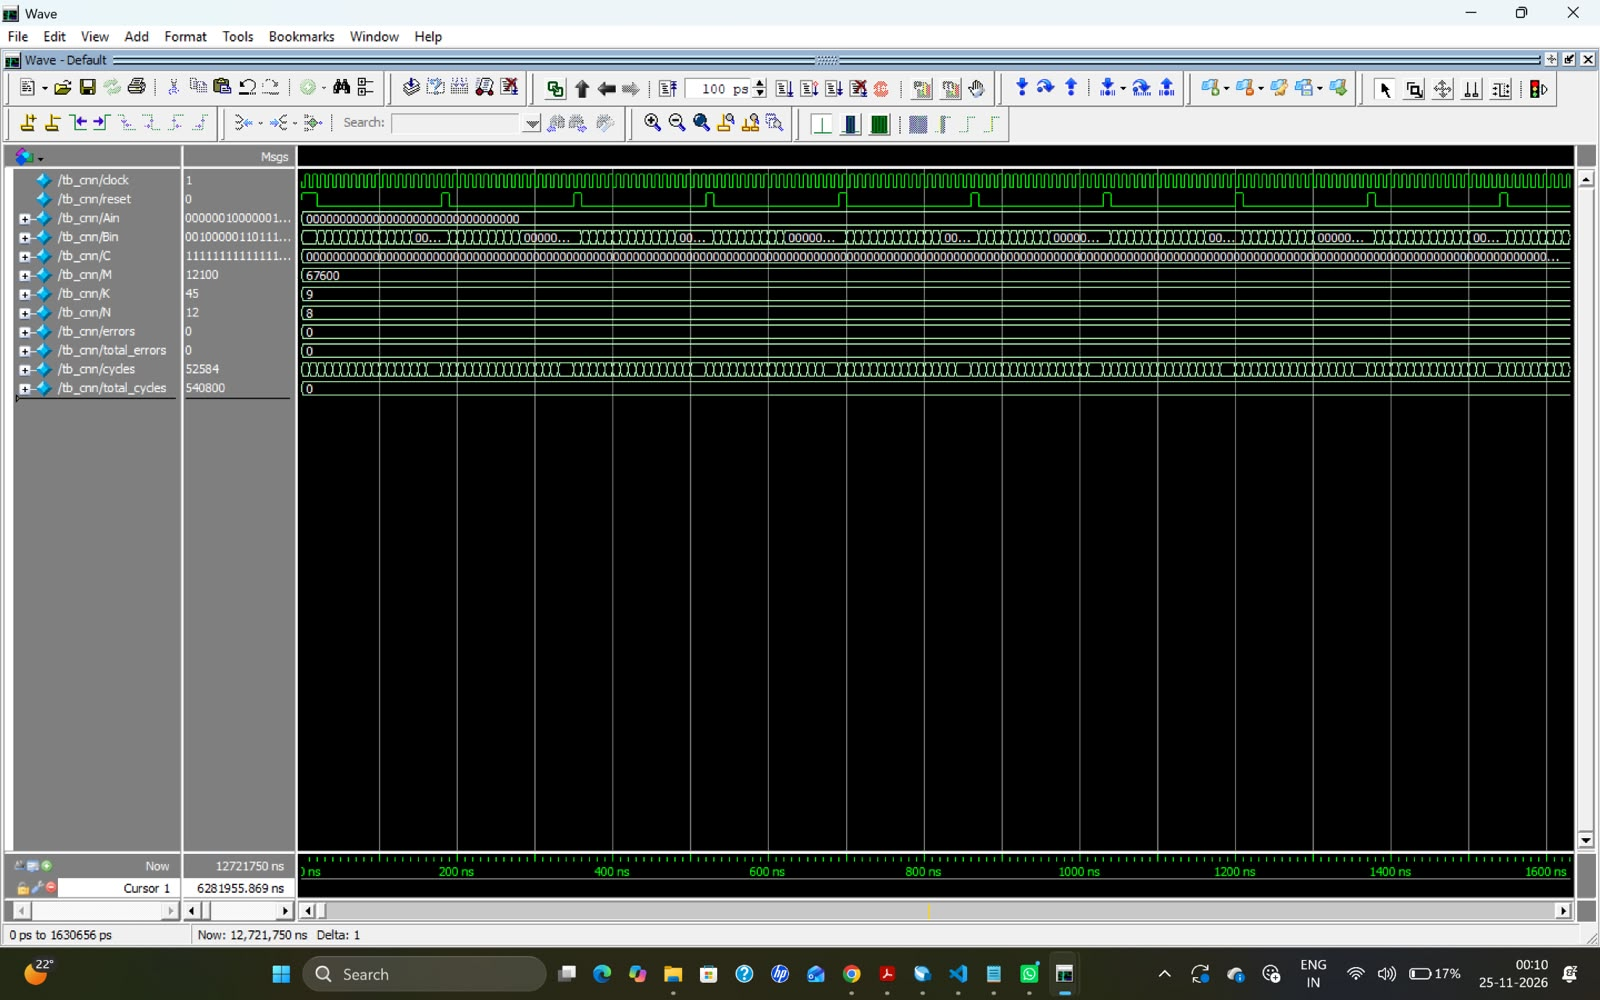
\includegraphics[width=\textwidth]{figures/cnn_modelsim.jpeg}
\caption{Teammate-provided ModelSim screenshot for Part C(ii), reproduced
as received. The displayed matrix-error counters are zero. This image
contains no final classification-accuracy result.}
\label{fig:cnn_modelsim}
\end{figure*}

\begin{figure*}[t]\centering
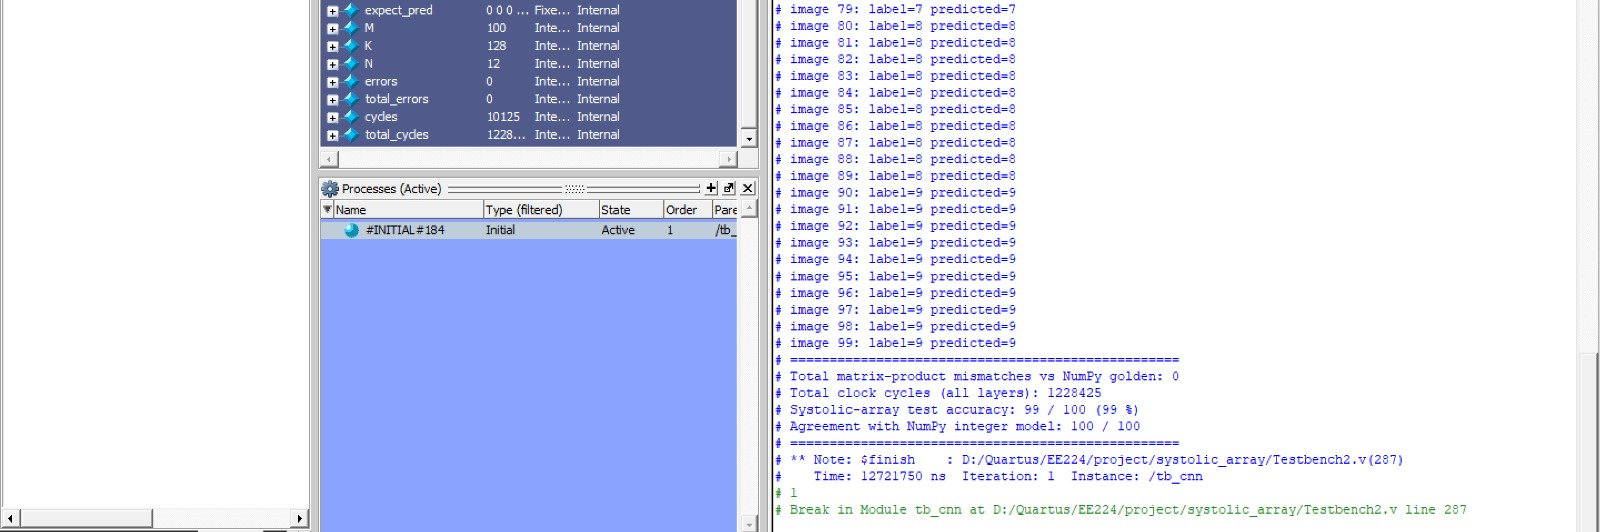
\includegraphics[width=\textwidth]{figures/cnn_modelsim_summary.jpeg}
\caption{Teammate-provided final ModelSim transcript. It reports zero
matrix-product mismatches, 1,228,425 total clock cycles, 99/100 test accuracy,
and 100/100 agreement with the NumPy integer model. The displayed transcript
ends with the testbench's \code{$finish} call.}
\label{fig:cnn_summary}
\end{figure*}


\section{Reproduction and completion}
Run the first three cells of \code{python/cnn_part1.ipynb} in order in an
environment with TensorFlow, NumPy, and Matplotlib. The output directory is
relative to the notebook's working directory. Compile both RTL files and
the shared driver together with the desired SystemVerilog testbench top.
The clocks have a 10\,ns period; this is a simulation stimulus setting,
not a measured maximum hardware clock frequency. The CNN top accepts
\code{+DATA_DIR=path/to/modelsim_data}. The optional \code{+VCD} switch
enables waveform dumping.

The Part A/B local simulation results and the supplied Part C waveform
and final summary are included in this report. The named PDF includes
all three members' names as requested by the question paper. No FPGA
synthesis, timing closure, or physical speedup claim is made in this report.

\begin{thebibliography}{9}
\bibitem{question} EE224 Digital Systems. \emph{Course Project Question Paper:
Implementing Inference for Convolutional Neural Networks through Systolic
Arrays}. Semester 1, 2026--2027. Supplied course document.
\bibitem{repo} Torque42. \emph{ee224-cnn-systolic-array}. Base commit
\code{70a34f2}, with local working changes. Source and saved notebook outputs:
\url{https://github.com/Torque42/ee224-cnn-systolic-array}.
\end{thebibliography}

\clearpage\onecolumn\appendix
\section{Numerical reference matrices}\label{app:matrices}
The following matrices are generated from the exact deterministic formulas
used in \code{tb_systolic_array.sv}. Their products were calculated separately
using scalar integer dot products. Every entry below also matches the
recorded behavioural simulation; the VCD-derived summary is stored in
\code{report/simulation/results.json}.
\subsection{\texorpdfstring{$K=4$, seed $s=1$}{K=4, seed 1}}
\[
A_4=\begin{bmatrix}-127&-120&-113&-106\\-98&-91&-84&-77\\-69&-62&-55&-48\\-40&-33&-26&-19\end{bmatrix},\quad
B_4=\begin{bmatrix}-125&-94&-63&-32\\-114&-83&-52&-21\\-103&-72&-41&-10\\-92&-61&-30&1\end{bmatrix}.
\]
\[
A_4B_4=\begin{bmatrix}50946&36500&22054&7608\\38360&27510&16660&5810\\25774&18520&11266&4012\\13188&9530&5872&2214\end{bmatrix}.
\]
For example, $C_{00}=(-127)(-125)+(-120)(-114)+(-113)(-103)+(-106)(-92)=50{,}946$.
\subsection{\texorpdfstring{$K=8$, seed $s=9$}{K=8, seed 9}}
\[
A_8=\begin{bmatrix}-119&-112&-105&-98&-91&-84&-77&-70\\-90&-83&-76&-69&-62&-55&-48&-41\\-61&-54&-47&-40&-33&-26&-19&-12\\-32&-25&-18&-11&-4&3&10&17\end{bmatrix}.
\]
\[
B_8=\begin{bmatrix}-101&-70&-39&-8\\-90&-59&-28&3\\-79&-48&-17&14\\-68&-37&-6&25\\-57&-26&5&36\\-46&-15&16&47\\-35&-4&27&58\\-24&7&38&69\end{bmatrix}.
\]
\[
A_8B_8=\begin{bmatrix}50484&27048&3612&-19824\\35984&19740&3496&-12748\\21484&12432&3380&-5672\\6984&5124&3264&1404\end{bmatrix}.
\]

\section{Complete synthesizable Verilog}\label{app:rtl}
These listings are read directly from the implementation files when the
report is compiled. Operands are signed, and each output accumulator is
24 bits wide at the default configuration.
\lstinputlisting[language=Verilog,title={Processing element: processing\_element.v}]{../verilog/processing_element.v}
\lstinputlisting[language=Verilog,title={Structural array: systolic\_array.v}]{../verilog/systolic_array.v}

\clearpage
\section{Complete SystemVerilog testbenches}\label{app:tests}
The shared driver implements skewed stimulus, tile resets, per-edge
scoreboarding, and collection of DUT results. It is verification code and
is not intended for synthesis. The small testbench tops select the Part A
and Part B scenarios; the CNN top performs the Part C(ii) layer chain.
\lstinputlisting[language=Verilog,title={Shared driver: systolic\_test\_driver.sv}]{../verilog/tb/systolic_test_driver.sv}
\lstinputlisting[language=Verilog,title={Part A: tb\_processing\_element.sv}]{../verilog/tb/tb_processing_element.sv}
\lstinputlisting[language=Verilog,title={Part B: tb\_systolic\_array.sv}]{../verilog/tb/tb_systolic_array.sv}
\lstinputlisting[language=Verilog,title={Part C(ii): tb\_cnn\_inference.sv}]{../verilog/tb/tb_cnn_inference.sv}
\end{document}
